\section{Experiments}
\label{sec:experiments}

Say you are hosting an elegant dinner party, and wish to select a balanced set of wines for drinking and flowers for decoration.
We demonstrate \tsip~ and \greedy~ on the Iris and Wine datasets \citep{misc_iris_53, misc_wine_109, scikit-learn}.
This has an intuitive interpretation as selecting diverse elements that reflects the peculiar structure of the diversification problem.
Features like \textit{ petal width} are rows in $X$.
They are features on the basis of which we may select among the flowers those which are most distinct from another.
Thus, in diversification, $P = n$.

%add description of words
\begin{figure}[t]
   \centering
    % Row 1: Wine and Iris
    \begin{subfigure}[b]{0.45\textwidth}
        \centering
        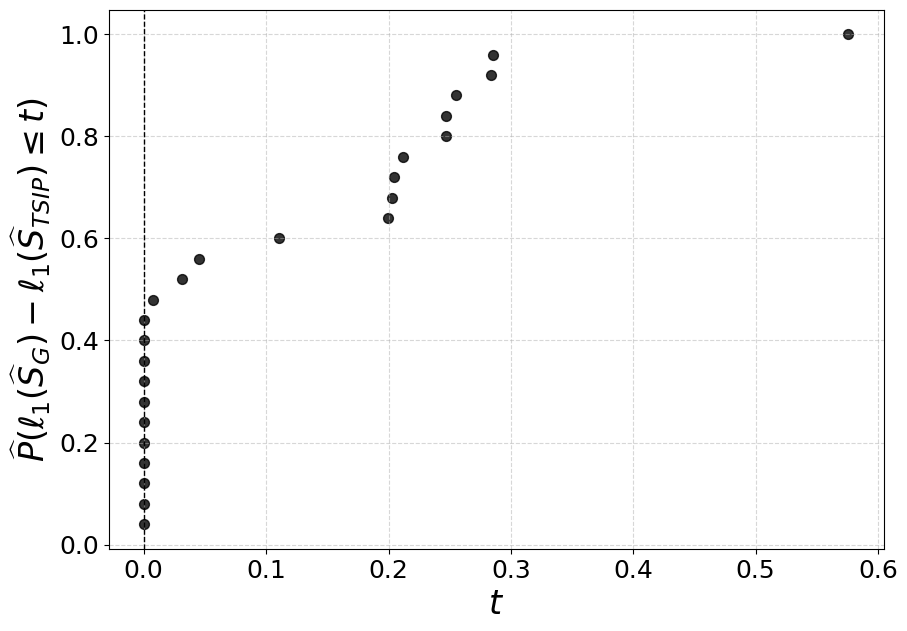
\includegraphics[width=\textwidth]{../figures/wine_standardized_isometry_losses_ecdf}
        \caption{Wine}
        \label{fig:wine_isometry_losses}
    \end{subfigure}
    \hfill
    \begin{subfigure}[b]{0.45\textwidth}
        \centering
        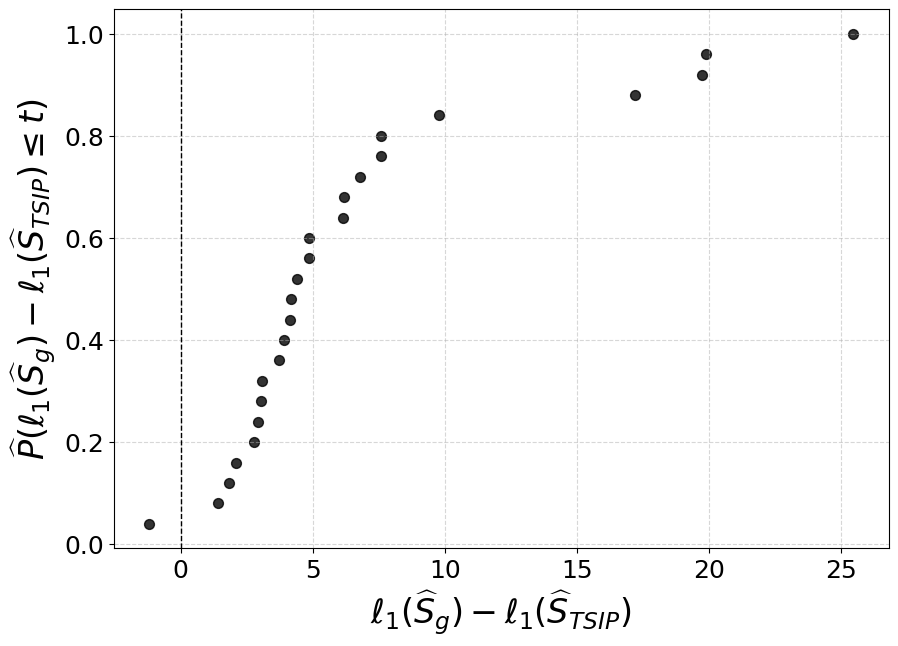
\includegraphics[width=\textwidth]{../figures/iris_standardized_isometry_losses_ecdf}
        \caption{Iris}
        \label{fig:iris_isometry_losses}
    \end{subfigure}

    \vspace{1em}

    % Row 2: Ethanol and Words
    \begin{subfigure}[b]{0.45\textwidth}
        \centering
        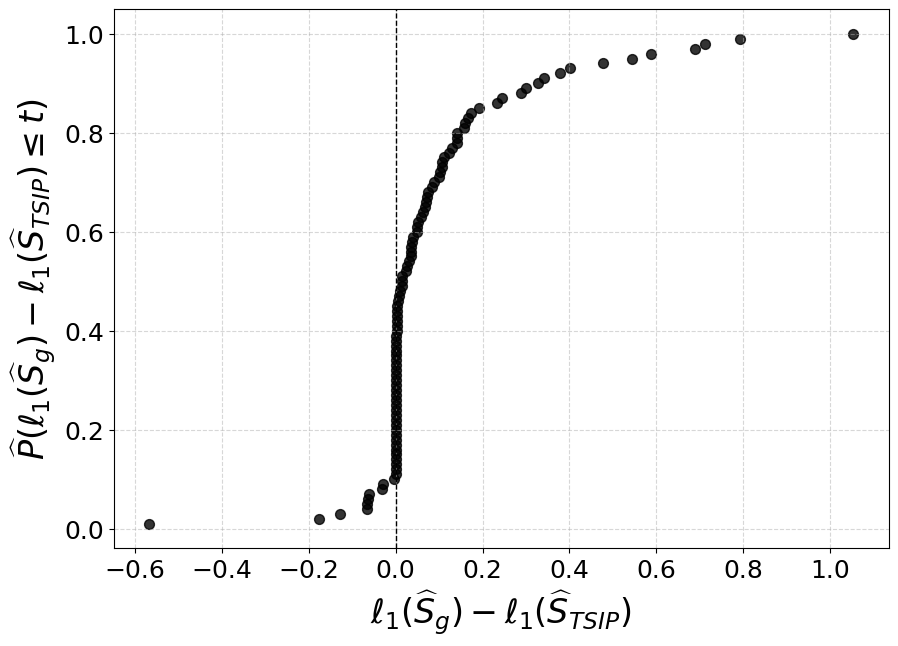
\includegraphics[width=\textwidth]{../figures/ethanol_isometry_losses_ecdf}
        \caption{Ethanol}
        \label{fig:ethanol_isometry_losses}
    \end{subfigure}
    \hfill
    \begin{subfigure}[b]{0.45\textwidth}
        \centering
        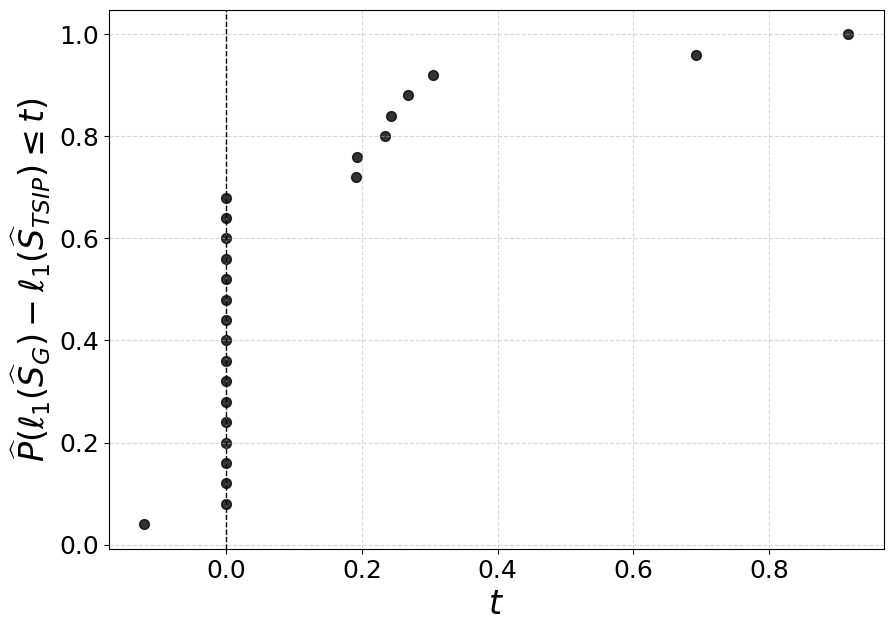
\includegraphics[width=\textwidth]{../figures/words_ecdf}
        \caption{Words}
        \label{fig:words_isometry_losses}
    \end{subfigure}
    \caption{Empirical cumulative distributions of isometry losses $\ell_1(\widehat{S}_g) - \ell_1(\widehat{S}_{TSIP})$ for Wine, Iris, Ethanol, and Words datasets across $R$ replicates.
    The distributions reflect the relative $\ell_1$ losses of the supports estimated by greedy optimization on the $\ell_1$ objective is less than or equal to $\ell_1$ loss of the support estimated by \tsip.
    As shown here and detailed  in Table \ref{tab:experiments}, losses are generally lower for two-stage isometry pursuit solutions.}
    \label{fig:isometry_losses}
\end{figure}

Our main interpretability dataset is the Ethanol dataset from \citet{Chmiela2018-at, Koelle2022-ju}.
Tather than selecting between bourbon and scotch we evaluate a dictionary of interpretable features  - bond torsions - for their ability to parameterize the molecular configuration space.
In this interpretability use case, columns denote gradients of informative features.
We compute Jacoban matrices of putative parametrization functions and project them onto estimated tangent spaces (see \citet{Koelle2022-ju} for preprocessing details).
Rather than selecting between data points, we are selecting between functions which parameterize the data.
This dataset exemplifies our motivating example - the search for locally isometric embeddings.

We also construct a small word embedding dataset.
%Mikolov2013-lt not showing
Inspired by the linear representation hypothesis \citep{Park2023-hq} and the construction over complete dictionaries of concepts in representation space \citep{templeton2024scaling, Makelov2024-bw}, we apply isometric pursuit to prune down embeddings of concept dictionaries into their basis components.
As with the other datasets, we measure success primarily numerically against the ground truth objective values obtained by greedy solutions.
Further details on this dataset are given in Section \ref{sec:word_embeddings}.

\begin{table}[t]
\tiny
\centering
\begin{tabular}{|c|c|c|c|c|c|c|c|c|c|c|}
\toprule
Name & $D$ & $P$ & $R$ & $c$ & $\ell_1(X_{.\widehat{S}_{G}})$ & $|\widehat{S}|$ & $\ell_1(X_{.\widehat{S}})$ &
\begin{tabular}{c}
$\widehat P (\ell_1(X_{.\widehat{S}_{G}}) >$ \\
$\ell_1(X_{.\widehat{S}}))$
\end{tabular} &
\begin{tabular}{c}
$\widehat P (\ell_1(X_{.\widehat{S}_{G}}) =$ \\
$\ell_1(X_{.\widehat{S}}))$
\end{tabular} &
\begin{tabular}{c}
$\widehat P(\bar{\ell}_1(X_{.\widehat{S}_{G}}) >$ \\
$\bar{\ell}_1(X_{.\widehat{S}}))$
\end{tabular} \\
\midrule
Iris & 4 & 75 & 25 & 1 & 14 ± 7.3 & 6.7 ± 1 & 6.9 ± 1.4 & 0.96 & 0 & 2.4e-05 \\
Wine & 6 & 89 & 25 & 1 & 7.7 ± 0.33 & 13 ± 1.5 & 7.6 ± 0.29 & 0.64 & 0.16 & 6.3e-04 \\
Ethanol & 2 & 756 & 100 & 1 & 2.6 ± 0.3 & 90 ± 1.7e+02 & 2.5 ± 0.2 & 0.66 & 0.17 & 2.1e-05 \\
Words & 6 & 61 & 25 & 1 & 14 ± 1.3 & 11 ± 1.3 & 14 ± 1.2 & 0.52 & 0.12 & 2.1e-02 \\
\bottomrule
\end{tabular}
\caption{Experimental parameters and results.
For Iris, Wine, and Words, probability estimates $\widehat P$ result from random downsampling features $[P]$ by a factor of $2$ to create $R$ replicates, while for Ethanol, replicates correspond to individual data points.
Distributional probabilities $\widehat P (\ell_1(X_{.\widehat{S}_{G}}) > \ell_1(X_{.\widehat{S}_{TSIP}}))$ and $\widehat P (\ell_1(X_{.\widehat{S}_{G}}) = \ell_1(X_{.\widehat{S}_{TSIP}}))$ are empirical across replicates, while asymptotic probabilities $\widehat P(\bar{\ell}_1(X_{.\widehat{S}_{G}}) > \bar{\ell}_1(X_{.\widehat{S}_{TSIP}}))$ is computed by paired two-sample T-test on  $\ell_1(X_{.\widehat S})$ and $\ell_1(X_{.\widehat S_{G}})$.
For brevity, in this table $\widehat S := \widehat {S}_{TSIP}$.
}
\label{tab:experiments}
\end{table}

For basis pursuit, we use the SCS interior point solver \citep{ocpb:16} from CVXPY \citep{diamond2016cvxpy, agrawal2018rewriting}, which is able to push sparse values arbitrarily close to 0 \citep{cvxpy_sparse_solution}.
Statistical replicas for Wine, Iris, and Words are created by resampling across $[P]$.
Due to differences in scales between rows, these are first standardized.
For the Wine dataset, even \brute~ on $\widehat {S}_{IP}$ is prohibitive in $D=13$, and so we truncate our inputs to $D=6$.
For Ethanol, replicas are created by sampling from data points and their corresponding tangent spaces are estimated in $B = 252$.

Figure \ref{fig:isometry_losses} and Table \ref{tab:experiments} show that the $\ell_1$ accrued by the subset $\widehat S_{G}$ estimated using \greedy~ with objective $\ell_1$ is higher than that for the subset estimated by \tsip.
This effect is statistically significant across datasets.
Generally, the ground truth loss obtained by \greedy~ optimization of $\ell_1$ is higher and therefore worse than that obtained by two-stage isometry pursuit.
Table \ref{tab:experiments}  and Figure \ref{fig:support_cardinalities} detail intermediate support recovery cardinalities from \isometrypursuit.
Isometry pursuit substantially reduced the size of the dictionary and made brute search computationally feasible.
Wall-clock runtimes are given in Section \ref{sec:timing}.
However, the preferable performance of two-stage isometry pursuit is not robust to different choices of $c$ on the Wine dataset in Figure \ref{fig:stacked_power_comparison}.
These show that the preference for the two-stage isometry pursuit solution is strongest around $c=1$ and is consistent across feature truncation dimensions.

\clearpage

\begin{figure}[t!]
    \centering
    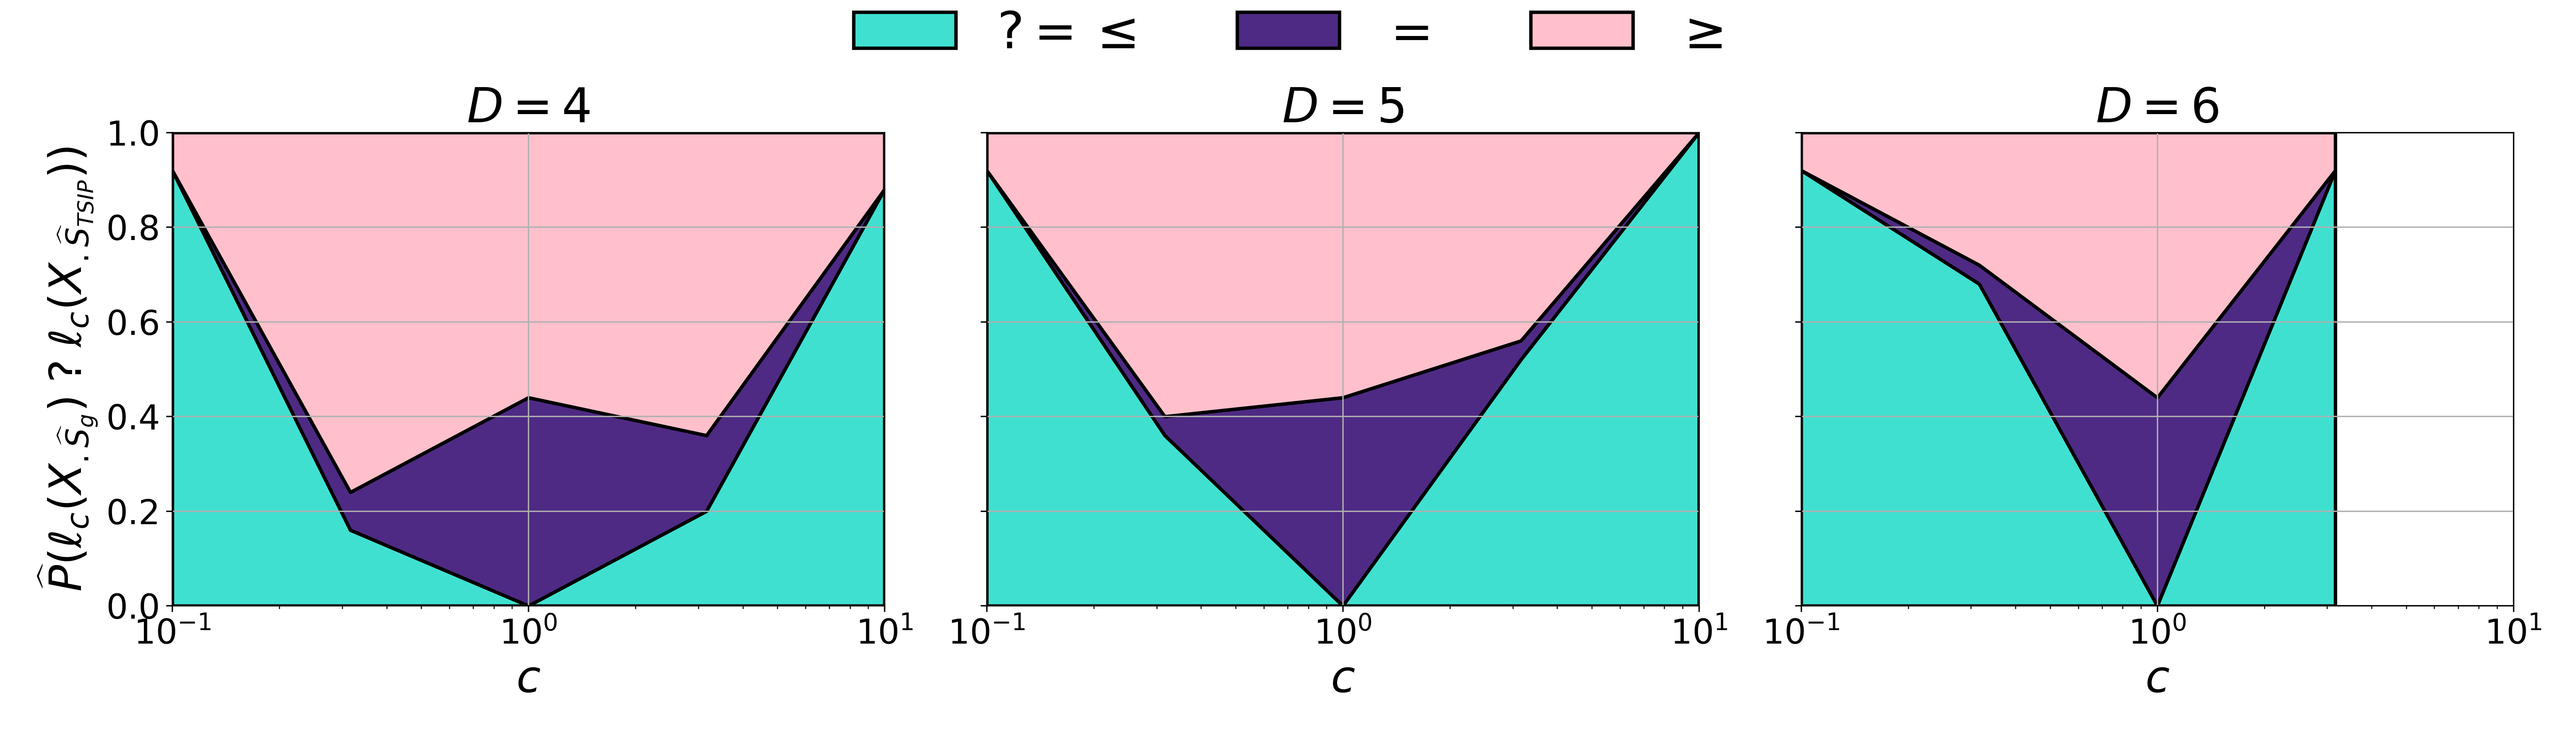
\includegraphics[width=\textwidth]{../figures/grid_power_comparison_filled.png}
    \caption{
        Proportions of support selection outcomes as power parameter $c$ varies, for different values of $D$ in the Wine dataset across various values of $c$.
        The turquoise area indicates when greedy solution  $\widehat{S}_G$ outperforms $\widehat{S}_{\text{TSIP}}$, purple shows ties, and pink indicates $\widehat{S}_{\text{TSIP}}$ is better.
        Solution at $c=10$ is not plotted for $D=6$ due to numerical overflow.
    }
    \label{fig:stacked_power_comparison}
\end{figure}



